\newcommand{\figureAnalogSignalExample}[1]{
  \begin{figure}[ht]
    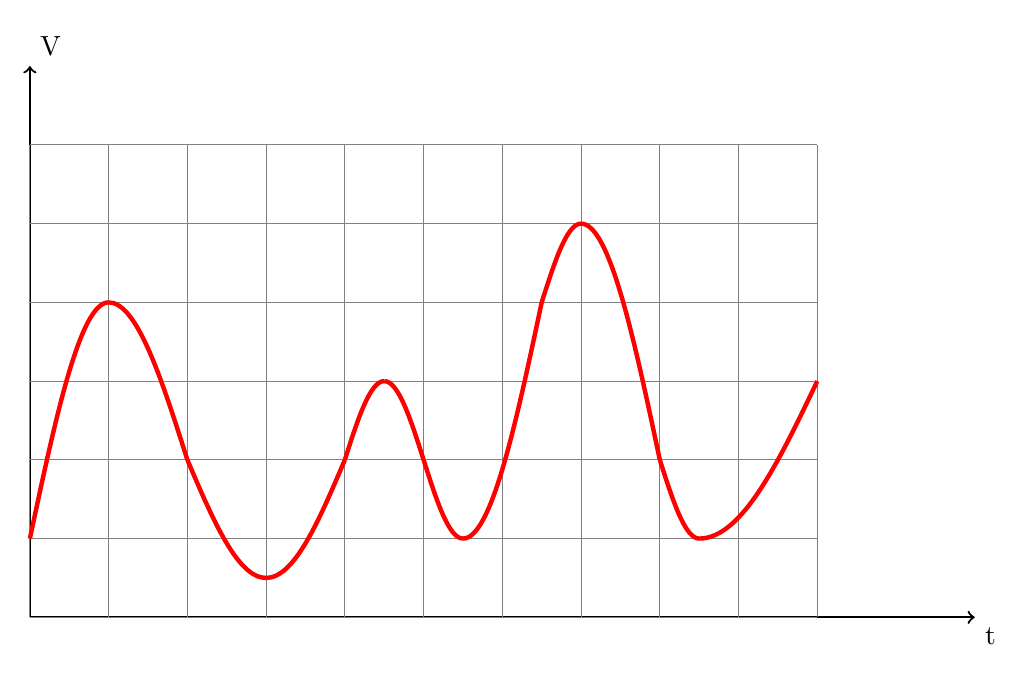
\begin{tikzpicture}
      \draw[thick, ->] (0, 0) -- (12, 0) node[anchor=north west] {t};
      \draw[thick, ->] (0, 0) -- (0,  7) node[anchor=south west] {V};
      \draw[gray] (0, 0) grid (10, 6);
      \draw[ultra thick, red] (0,1)   sin (1,4);
      \draw[ultra thick, red] (1,4)   cos (2,2);
      \draw[ultra thick, red] (2,2)   sin (3,0.5);
      \draw[ultra thick, red] (3,0.5) cos (4,2);
      \draw[ultra thick, red] (4,2)   sin (4.5,3);
      \draw[ultra thick, red] (4.5,3) cos (5,2);
      \draw[ultra thick, red] (5,2)   sin (5.5,1);
      \draw[ultra thick, red] (5.5,1) cos (6.5,4);
      \draw[ultra thick, red] (6.5,4) sin (7,5);
      \draw[ultra thick, red] (7,5)   cos (8,2);
      \draw[ultra thick, red] (8,2)   sin (8.5,1);
      \draw[ultra thick, red] (8.5,1) cos (10, 3);
    \end{tikzpicture}
    \caption{#1}
    \label{fig:adc-analog-signal-example}
  \end{figure}
}
